\documentclass[11pt,a4paper,ngerman,bibtotoc]{scrartcl}
\usepackage[utf8]{inputenc}
\usepackage[ngerman]{babel}
\usepackage[pdfpagelabels,pdfstartview = FitH,bookmarksopen = true,bookmarksnumbered = true,linkcolor = black,plainpages = false,hypertexnames = false,citecolor = black] {hyperref}
\usepackage[pdftex]{graphicx}
\usepackage{float} % to force figure at correct position
\usepackage{amsmath,amssymb}
\usepackage[style=ieee,backend=biber]{biblatex}
\bibliography{literature.bib}

% hyperlinks for figures % tables
\usepackage{prettyref}
\usepackage{hyperref}
\usepackage[all]{hypcap}%nach hyperref
\newrefformat{fig}{Abbildung~\ref{#1}}
\newrefformat{tab}{Tabelle~\ref{#1}}

\titlehead{
	\begin{minipage}{7.6cm}
		\vspace{-6mm}
		\hspace{-4mm}
  	
\includegraphics[scale=0.4]{bilder/fu_logo_header.jpg} % Hochschullogo
	\end{minipage}
	\begin{minipage}{7.6cm}
		\begin{flushright}
			Fachbereich Mathematik und Informatik\\
			Institut für Informatik\\
			Softwareprojekt Mobilkommunikation\\
		\end{flushright}
	\end{minipage}
	\\\\
	\centerline{\hrulefill}
}%end of titlehead
\title{
	\vspace{10mm}
	Hintergrundenfernung auf Basis von Hidden Markov Models\\
	\vspace{10mm}
	
\includegraphics{bilder/fu_logo.png}	%  kleines logo
	\vspace{10mm}
}
\author{Marcin Nawrocki\\Patrick Mertes\\Hinnerk van Bruinehsen\\\\\\Betreuer: Alexandra Danilkina\\\\}
\date{28. Februar 2014}
%\today

\begin{document}
\maketitle\thispagestyle{empty}
\newpage
\tableofcontents
\listoffigures	% to include list of figures in content
\newpage

\section{Einleitung}
\label{chap:einleitung}

Dieses Kapitel gibt eine Einführung in das Projekt SAFEST\cite{safest} und erläutert die vorliegende Problemstellung, welche im Rahmen des Softwareprojektes Mobilkommunikation im Wintersemester 13/14 bearbeitet wurde.


\subsection{Kontext und Motivation}
\label{sec:motivation}

SAFEST\cite{safest} ist ein deutsch-französisches Projekt mit der Zielsetzung, die Sicherheit an öffentlichen Plätzen und kritischen Infrastrukturen durch Realisierung eines Sensornetzwerkes mit Infrarotkameras zu erhöhen.
 Um dieses Ziel zu erreichen, überwacht das Sensornetzwerk ein vorgegebenes Areal und verarbeitet die gewonnenen Mittelinfrarotbilder mit Hilfe von Algorithmen in Hinblick auf verschiedene Parameter.
 Der eigentliche Gewinn an Sicherheit soll dadurch erfolgen, dass automatisiert auf Grundlage der ermittelten Parameter die Dichte der sich in dem Areal aufhaltenden Personen ermittelt wird, woraus wiederum ein Rückschluss auf die Wahrscheinlichkeit des Auftretens einer Massenpanik gezogen werden soll.\\
Der erste wichtige Schritt bei dieser Analyse ist die automatisiere Erkennung und Zählung von sich im Bildbereich befindlichen Personen.
 Um diesen Schritt zu ermöglichen, muss zunächst der Hintergrund vom Vordergrund des Bildes getrennt werden.
% Hintergrund ist in diesem Zusammenhang als der statische Teil des Bildes zu verstehen, wohingegen der Vordergrund die sich bewegendenden Personen sind.
% Durch die Verwendung einer Wärmebildkamera wird diese Trennung erst einmal erleichtert, da die relativ warmen Personen heller gefärbt sind als der relativ kalte Boden.
% Da der Hintergrund aber nicht total statisch ist und der Unterschied der Helligkeit stark von der Temperaturdifferenz zwischen Boden und Personen abhängt, wird die Trennung allerdings erschwert.
% Ein weiteres Problem ist die ständige Neukalibrierung der verwendeten Kamera.
% Diese findet statt, wenn sich das Wärmespektrum des beobachteten Areals stark ändert, so zum Beispiel wenn viele Personen in das Bild ein- oder austreten.\\
Die verwendete Kamera stellt wärmere Bereiche heller und kältere Bereiche dunkler dar. Daraus folgt, dass Personen erwartungsgemäß eher weiß und Hintergrund erwartungsgemäß eher schwarz dargestellt werden.
Allerdings kalibiert sich die Kamera regelmäßig neu, um den gesamten Graustufenverlauf zur darstellung der Wärme zu nutzen. Daraus folgt, dass mitunter auch sehr kalte Bereiche sehr hell dargestellt werden, wenn diese die wärmsten von der Kamera erfassten Temperaturen besitzen.
Aus dieser Eigenschaft der Kamera folgt somit auch, dass ein naiver Ansatz wie eine feste Zuordnung von Temperatur und Graustufenwert nicht möglich ist. Ein weiteres Hindernis bei der einfachen Zuordnung von Temperaturwerten zu Vorder- oder Hintergrund ist die Tatsache, dass Kleidung (besonders zum Beispiel dickere Jacken) die Temperatur sehr gut nach außen isolieren und damit Teile von Personen sehr dunkel auf dem Kamerabild erscheinen lassen.\\
Die Trennung von Vorder- und Hintergrund kann daher nicht allein aufgrund der dargestellten Temperatur erfolgen, sondern muss als zweiten Faktor die Bewegung mit einbeziehen.
Personen sind also in der Darstellung der Regel nach helle, bewegte Objekte.\\
Nach erfolgter Entfernung des Hintergrunds folgt als nächster Schritt in der Analyse die automatisierte Bestimmung der auf dem Bild sich befindlichen Personen.
Wird diese Analyse erfolgreich ausgeführt, so muss nur noch dieser Wert an eine Kontrolleinheit übertragen werden, nicht aber das eigentliche Bild, was im Hinblick auf auf den Datenschutz sehr wichtig ist.\\
Eigentlich für Objekterkennung bewährte Algorithmen wie Histogramm orientierte Gradienten (HOG)\cite{Dalal05histogramsof} und die Mischung gausscher Verteilungsdichten (MOG)\cite{DBLP:conf/focs/Dasgupta99}, können sich auf die Eigenschaften von Vorder- und Hintergrund, insbesondere die durch die Kamerakalibrierung entstehende Dynamik, nicht so einstellen, dass sie befriedigende Ergebnisse liefern.

Daher soll ein neuer Algorithmus entwickelt und evaluiert werden, der über die Fähigkeit verfügt, sich der Dynamik anzupassen, um das Problem zu lösen.\\


\subsection{Aufgabenbeschreibung}
\label{sec:aufgabenbeschreibung}

Das Ziel unseres Softwareprojektes ist es, ein Verfahren zu entwickeln, welches das Bild einer Infrarotkamera in Vorder- und Hintergrund trennt.
 Die genauen Anforderungen für diesen Prozess werden in Kapitel \ref{sec:anforderungsanalyse} beschrieben.
 Hierbei soll die allgemeine Verwendbarkeit von Hidden-Markov-Modellen(HMM)\cite{Stamp04arevealing} und der Diskreten Kosinustransformation(DCT)\cite{Khayam03thediscrete} gezeigt werden.
 Die theoretischen Grundlagen werden hierzu im Kapitel \ref{chap:entwurf} ff. erläutert.
 Schlussendlich soll eine vergleichende Evaluation durchgeführt werden, in dem das entwickelte Verfahren gegen ein bereits vorliegendes Histrogramm-basiertes Verfahren antreten muss(vgl. Kapitel \ref{chap:evaluation}).\\
Da bereits ein Algorithmus zum Zählen von Personen vorliegt, muss dieser nicht innerhalb dieses Projektes entworfen beziehungsweise implementiert werden.


\section{Entwurf eines Vordergrund-Extraktors}
\label{chap:entwurf}

In diesem Kapitel wird der nötige, theoretische Hintergrund herausgearbeitet und unser Entwurf gemäß den Anforderungen vorgestellt.
Es wird das Konzept der Hidden-Markov-Modelle (HMM) und der Diskreten Kosinustransformation(DCT) erläutert und deren Verknüpfung eingeführt.
%TODO: Kommentar unklar: "mit fehlenden werten pro pixel ..."


\subsection{Anforderungsanalyse}
\label{sec:anforderungsanalyse}

Die funktionalen Anforderungen an einen Vordergrund-Extraktor sind bereits in der Aufgabenbeschreibung (\ref{sec:aufgabenbeschreibung} ausgeführt:
Es soll demonstriert werden, dass HMM zur Trennung von Vordergrund und Hintergrund bei stark heterogenen Hintergründen geeignet sind, wie in folgender Abbildung dargestellt:
%TODO: Abb einfügen

Die nichtfunktionalen Anforderungen umfassen vor allem eine einfache Benutzbarkeit durch Automatisierung.
Der Ressourcenbedarf soll möglichst gering sein - ein Video wird für gewöhnlich mit 25 Frames pro Sekunde aufgezeichnet, im Idealfall ist eine optimale Analyse jedes einzelnen Frames in Echtzeit möglich.
%Hierbei ist zu beachten, dass eine hohe Korrektheit zu erzielen ist, das heißt, dass die Ergebnisse fehlerfrei sein müssen.
Allerdings ist zu berücksichtigen, dass eine möglichst hohe Korrektheit wichtiger ist, als eine Analyse in Echtzeit. Falls nötig können auch Bilder ausgelassen werden.
%Eine Flexibilität bezüglich unterschiedlicher Videotypen ist gewünscht, also die Unterstützung von variierenden Videoauflösungen et cetera.
Die Analyse sollte jedoch unabhängig von den Parametern des verwendeten Videomaterials wie beispielsweise unterschiedliche Videoformate oder Auflösungen statt finden.


\subsection{Hidden-Markov-Modelle}
\label{sec:hiddenmarkovmodel}

Die Markov Modelle stammen aus der Wahrscheinlichkeitstheorie und entsprechen einem stochastischem Zustandsautomaten, bei dem die Zustandswechsel gemäß einer Wahrscheinlichkeit statt finden und nicht abhängig von der Vergangenheit sind, sondern nur von dem aktuellen Zustand.
%TODO: Kommentar: etwas salopp formuliert: sollte also nochmal überarbeitet werden.
Bei den HMM\cite{Stamp04arevealing} können jene Zustände nicht beobachtet werden, sondern nur die Beobachtungen/Ausgaben, welche während dieses Zustandes auftreten, sie werden Emissionen genannt.
Die Zustandsübergangswahrscheinlich- keiten sind in den HMM somit nicht die einzigen Parameter, die Emissionswahrscheinlichkeiten bilden die zweiten Parameter.\\

Formal definiert ist ein HMM ein 5er-Tupel $\lambda= (S, V, A, B, \Pi)$ mit:

\begin{itemize}
 \item $S = {s_1,..., s_n}$ sei die Menge aller Zustände
 \item $V = {v_1,..., v_m}$ das Alphabet der möglichen Emissionen
 \item $A \in \mathbb{R}^{n \times n}$ sei eine Übergangsmatrix zwischen den Zuständen, $a_{ij}$ entspricht der Wahrscheinlichkeit des Übergangs von Zustand $s_i$ in Zustand $s_j$
 \item $B \in \mathbb{R}^{n\times m}$ sei eine Beobachtungsmatrix, wobei $b_i(v_j)$ die Wahrscheinlihkeit angibt, im Zustand $s_i$ die Beobachtung (Emission) $v_j$ zu sehen
 \item $\Pi \in R^n$ die Initialverteilung, $\Pi_i$ sei die Wahrscheinlichkeit, dass $s_i$ der Startzustand ist
\end{itemize}

Ein HMM heißt zeitinvariant, wenn sich die Übergangs- und Emissionswahrscheinlichkeiten nicht mit der Zeit ändern.

HMM werden zunehmend in der Literatur zur Sprach-, Schrift und Mustererkennung \cite{Gales:2007:AHM:1373536.1373537}\cite{Yang1995161} verwendet, da sie mit den probabilistischen Übergängen die Prozesse der echten Welt besser widerspiegeln als deterministische Definitionen, zu dem können die Parameter durch Lernalgorithmen automatisiert bestimmt werden.
 siehe hierzu Kapitel 2.5.

%TODO: Grafik einfügen



Die vorliegende Abbildung demonstriert ein HMM mit 3 Zuständen und 4 Emissionen, wobei der Übergang aus jedem Zustand zu jedem Zustand und zusätzlich in jedem Zustand jede Emission möglich ist.
Es liegt eine Gleichverteilung vor, Übergänge zwischen Zuständen haben stets die Wahrscheinlichkeit $1/3$, die Emissionen haben stets eine Wahrscheinlichkeit von $1/4$.
 Beschriftung der Kanten aus Übersichtsgründen nicht dargestellt.
%TODO: Bedeutung von Beispiel/Grafik, wieso gleichverteilt, Quelle?


\subsection{Standartalgorithmen von HMMs}
\label{sec:standartalgorithmenHMM}
%TODO: Alexandras Vorschlag: Gängige Problemstellungen

Für die HMM wurden bereits viele Algorithmen entwickelt, welche Standardprobleme lösen.
 Die zwei häufigsten Problemstellungen bei HMMs sind das Lernproblem und das Evaluations-/Decodingproblem.

\begin{enumerate}
	\item Das Lernproblem bezieht sich auf die Problematik ein HMM so zu trainieren, dass man im Folgenden das HMM dafür nutzen kann, Aussagen über die wahrscheinlichsten Folgezustände zu treffen.
Gelöst wird dieses Problem durch den Baum-Welch Algorithmus, welcher dazu verwendet wird, unbekannte Parameter, genauer die Übergangs- und Emiossionswahrscheinlichkeiten eines HMM, zu bestimmen.
 Hierbei handelt es sich um einen erwartungsmaximierenden Algorithmus, welcher anhand von übergebenen Trainingssequenzen die Maximum-Likelihood-Schätzwerte berechnet.
 Die initialen Werte eines HMMs müssen geschätzt werden, hier wird für gewöhnlich eine Gleichverteilung angenommen, dass heißt das jeder Übergang und jede Emission in einem Zustand gleich wahrscheinlich sind.

	\item Das Evaluations-/Decodingproblem bezieht sich auf die Problemaik aus den verschieden Wahrscheinlichkeiten Aussagen über die Folgezustände oder aber über die Wahrscheinlichkeit bestimmter Zustandsketten zu treffen.
Es wird durch den Forward-Algorithmus beziehungsweise den eng verwandten Viterbi-Algorithmus gelöst.
 Gegeben sei eine Chronik an k-letzten Emissionen, was ist die Wahrscheinlichkeit für eine bestimme Emission? Und ferner, was ist die wahrscheinlichste Emission? Der Viterbi-Algorithmus berechnet zur Beantwortung dieser Frage die wahrscheinlichste Zustandssequenz, also eine Sequenz die die Wahrscheinlichkeit der übergebenen Emissionssequenz maximiert, und kann anhand des letzten Zustandes dieser Sequenz das Problem lösen.
 Der Forward-Algorithmus ist ein Algorithmus aus der dynamischen Programmierung und optimiert im Gegensatz zum Viterbi nicht rückwirkend die gesamte Zustandssequenz neu, sondern berechnet den aktuell wahrscheinlichsten Zustand auf Basis der zuvor berechneten Zustände und hängt diesen an.
 Somit ist der Forward Algorithmus zur Laufzeit grundsätzlich schneller, jedoch nicht so genau wie der Viterbi-Algorithmus.
 \end{enumerate}


\subsection{Diskrete Kosinustransformation}
\label{sec:dct}

Die Diskrete Kosinustransformation (DCT)\cite{Khayam03thediscrete} ist ein Verfahren, welches zur verlustbehafteten Kompression von Daten verwendet wird, wobei die bekannteste Anwendung das Dateiformat JPEG ist.
 Ähnlich zu der diskreten Fourier Transformation wird eine Information mittels Frequenzen repräsentiert, wobei wie der Name bereits nahe legt nur Kosiunusfunktionen verwendet werden.


Es existieren mehrere Varianten der DCT.
Wird jedoch die DCT auf Bildinformationen angewandt, speziell bei der JPEG-Kompression, so wird die zwei-dimensionale Typ II DCT verwendet, welche die gängiste Variante ist.
%TODO: Anmerkung: wieso ist DCT-II die gängigste Variante?
Die DCT erhält eine $n \times  n$ Matrix und gibt eine Matrix der selben Größe zürück, wobei im JPEG-Standard $8 \times 8$ Pixel Matrizen betrachtet werden.
Hierbei wird das Element $[1,1]$ als DC-Wert bezeichnet und bildet den Durchschnittswert der Farben der betrachteten Matrix; die restlichen 63 Werte der Matrix sind ein Offset zu dem DC-Wert und kodieren somit den Unterschied zum DC-Wert innerhalb der Matrix.
Diese Werte werden als AC-Werte bezeichnet.


Formal definiert ist die DCT eine lineare, invertierbare Funktion $f : \mathbb{R}^n \rightarrow \mathbb{R}^n$, welche $N$ reellwertige Werte aus $x[n]$ in $N$ reellwertige Werte nach $X[n]$ überführt:

 $X_k = \sum\limits_{n=0\rightarrow N-1} x_n \cos [\frac{\Pi}{N} + (n + \frac{1}{2}) k ]$ mit $k = 0,..., N-1$


Die folgende Abbildung zeigt das Ergebnis nach der Anwendung der DCT mit Einfärben der gesamten Blöcke in die jeweils berechneten DC-Werte.
%TODO: Abb einfügen, Name & Ref im Text einfügen.


\subsection{Modellierung eines Eingabealphabets}
\label{sec:modellierungeingabealphabet}

In unserem Projekt sollen HMM benutzt werden, um eine Entscheidung zu treffen, ob ein Bildbereich zum Vorder- oder zum Hintergrund gehört.
Nach dem das generelle Konzept von HMM in Kapitel \ref{sec:hiddenmarkovmodel} vorgestellt wurde, fehlt jedoch noch die Definition, wie eine Emission aussieht.
Das Alphabet der Emissionen wird als Eingabealphabet bezeichnet, da mit dessen Hilfe das System beschrieben werden kann.
Hierbei ist zu beachten, dass das Eingabealphabet endlich und diskret sein muss.
Zusätzlich sollte das Eingabealphabet aus möglichst wenigen, aussagekräftigen Symbolen bestehen.
Die Kodierung, also die Zuordnung von Daten zu bestimmten Emissionen,  eines Eingabealphabets gehört daher in unserem Fall zu der Kernleistung bei der Verwendung von HMM.\\
Die im Kapitel \ref{sec:standartalgorithmenHMM} vorgestellte DCT wird von uns verwendet, um ein Eingabealphabet zu erzeugen, wobei wir die DCT auf fest definierte Bereiche anwenden.
 Wir übernehmen die aus der Bildkompression üblichen 8 x 8 Pixelblöcke zur Einteilung des vorliegenden Bildes, da wir dieses als optimalen Kompromiss zwischen einer zu hohen und niedrigen Granularität ansehen: kleinere Betrachtungen, so zum Beispiel pixelbasierte Verfahren, wären deutlich rechenintensiver und anfälliger auf Bildrauschen und würden daher keine akkuraten Rückschlüsse bei Veränderungen des Pixelwertes ermöglichen.
 Bei größeren Betrachtungen wären relevante Veränderungen deutlich schwerer wahrzunehmen, speziell im DC-Wert, da dieser stets den Mittelwert aller Subpixel der Matrix darstellt.


\subsubsection{DC-Wert}

Da Bildaufnahmen von Mittelinfrarot-Kameras stets schwarzweiß sind (und warme Bereiche heller dargestellt werden als kühle) besitzt ein Pixel genau einen Informationskanal mit einem Grauwert zwischen 0 (schwarz) bis 255 (weiß).
Der DC-Wert liegt somit als Mittelwert ebenso in diesem Intervall.
Dieser Bereich ist zu groß um als Eingabealphabet für das HMM dienen zu können, da zum Beispiel der Übergang von einem Grauwert von 230 auf 235 nicht aussagekräftig ist, da es sich hierbei um Rauschen oder aber eine Neukalibrierung der Kamera, die sich ja stets auf die gesamte $8 \times 8$ Matrix auswirkt, halten kann.\\

Wir nehmen jedoch eine Dreiteilung des Wärmespektrums an, einen kühlen Hintergrund, warmen Vordergrund und ein mittelwarmen Bereich.
Diese Dreiteilung ergibt sich daraus, dass es sehr wahrscheinlich ist, dass sehr helle Bereiche zum Vordergrund und sehr dunkle Bereiche zum Hintergrund gehören.
Bei dem größten Bereich, der aus verschiedenen Grauwerten besteht, ist eine einfache Zuordnung allerdings nicht möglich. Mehr Teile machen hingegen auch keinen Sinn, da diese dann nur Zuordnungen wie "wahrscheinlich Vordergrund" oder "wahrscheinlich Hintergrund" zuliessen, diese Wahrscheinlichkeiten aber durch das HMM bereits mit einem unsicheren Teil abgebildet werden.
Histogramm-basierte Analysen der DC-Werte über mehrere unterschiedliche Videosequenzen über alle Pixelblöcke genormt bestätigen diese Annahme und manifestieren 3 Cluster, die wir vereinfacht Cluster schwarz, Cluster grau und Cluster weiß nennen - der Darstellungsfarbe des Wärmespektrums entsprechend.
Die Grenzen dieser Cluster sind abhängig von jedem Video und dem betrachteten Umfeld, denn die insbesondere die Kälte (und damit die Farbe) des Hintergrundes kann sich bei den jeweiligen Videos stark unterscheiden.


Wir bilden auf Basis dieser Erkenntnis die ersten 3 Symbole, wobei, wenn der DC-Wert eines Blockes in das Intervall eines Clusters fällt, wir die entsprechende Beobachtung erstellen:

\begin{itemize}
	\item DC-Wert im Intervall Cluster schwarz $\rightarrow$ Beobachtung: DC\_BLACK
	\item DC-Wert im Intervall Cluster grau$\rightarrow$ Beobachtung: DC\_GREY
	\item DC-Wert im Intervall Cluster weiß $\rightarrow$ Beobachtung DC\_WHITE
\end{itemize}

Das folgenden Bild zeigt eine exemplarische Einteilung in die drei Cluster.
 Die X-Achse beschreibt den Grauwert, die Y-Achse das Vorkommen.

%TODO: Grafik Histogramm einfügen, Achsenbezeichnungen, Name und Label ergänzen
 %
\subsubsection{AC-Wert}

Die bei der Anwendung der DCT entstehende 8 x 8 Matrix enthält 63 AC-Werte, diese bilden demnach den Großteil der in der Matrix kodierten Informationen; die Integration dieser Werte in das Eingabealphabet ist aufgrund der hohen Informationsdichte essenziell.\\
Eine Histogramm-basierte Betrachtung der AC-Werte analog zu der Betrachtung der DC-Werte ist nicht zielführend, da es sich hierbei um Offsets handelt, welche demnach im Histogramm ein Maximum um den Nullwert bilden.
Wir erkennen jedoch, das Menschen aufgrund ihrer warmen Austrahlung eine starke Kante zu dem Hintergrund bilden, läuft demnach ein Mensch durch einen Block, müsste eine deutliche Abweichung einiger AC-Werte zum DC-Wert entstehen.
Eine Block-basierte Analyse bestätigt diese Annahme, die Standardabweichung (STD) der AC-Werte bezüglich des DC-Wertes steigt deutlich an, falls eine Person sich im Block befindet beziehungsweise durch diesen hindurch läuft.


An folgender Abbildung sieht man auf der X-Achse den Zeitverlauf in Frame und auf der Y-Achse den Wert der Standardabweichung für den betrachteten Bock; es lässt sich feststellen, dass die Kurve der Standabweichung stark ausschlägt, falls eine Person durch den Block läuft.
%TODO: Abb einfügen, Name&Ref&Achsenbezeichnungen

Anhand von empirischen Tests lässt sich ein Threshold ermitteln, falls die Standardabweichung diesen übersteigt, befindet sich mit hoher Wahrscheinlichkeit eine Person im Block.
 In dem vorgestellten Beispiel liegt dieser bei 25.


Zusätzlich ist zu beachten, dass die Standardabweichung von wenigen, aber extremen statistischen Ausreißern kaum beeinflusst wird, diese Situation liegt  jedoch während der Erkennung von Menschen vor, insbesondere bei Personen, die Kleidung tragen, welche die Wärmeabgabe der Person dämmt, und dennoch einige freiliegende Körperteile sichtbar sind.
 In diesem Fall ist der Großteil der AC-Werte relativ klein und der DC-Wert des betrachteten Blockes für gewöhnlich innerhalb des grauen Intervalls.
 Um in diesen Situationen den Vordergrund besser zu erkennen, prüfen wir mithilfe eines selbstdefinierten Verfahrens outliers() ob stark-positive (warme) Ausreißer vorliegen, welches den Wahrheitswert true zurückliefert, falls eine gewissen Anzahl von Ausreißern erkannt wird.


Vor allem bei Kleidung tragenden Personen führt dies dazu, dass nicht nur ihre Körperkanten durch die STD erkannt werden, sondern jedoch auch die Körpermitte mathematisch erfasst wird.



Infolge dieser Erkenntnise bilden wir die zwei weiteren Beobachtungen:

\begin{itemize}
	\item $(\text{STD von }AC_{1-63} < \text{Threshold} ) \wedge !\text{Outliers} \rightarrow$  Beobachtung AC\_LOW
	\item $(\text{STD von }AC_{1-63} > \text{Threshold} ) \vee \text{Outliers} \rightarrow$  Beobachtung AC\_HIGH
\end{itemize}



Auf Basis unserer Beobachtungen können nun anhand aller möglichen Permutationen von DC- und AC-Beobachtungen die Symbole unseres Eingabealphabets gebildet werden. Diees ist in Tabelle \ref{table:eingabealphabet} dargestellt.

\begin{table}
	\label{table:eingabealphabet}
	\begin{center}
\begin{tabular}{|l|l|l|}
\hline
\textbf{Alphabetsymbol}&\textbf{DC-Wert}&\textbf{Standartabweichung AC}\\
\hline
Symbol 1&DC\_BLACK&AC\_LOW\\
\hline
Symbol 2&DC\_BLACK&AC\_HIGH\\
\hline
Symbol 3&DC\_GREY&AC\_LOW\\
\hline
Symbol 4&DC\_GREY&AC\_HIGH\\
\hline
Symbol 5&DC\_WHITE&AC\_LOW\\
\hline
Symbol 6&DC\_WHITE&AC\_HIGH\\
\hline
\end{tabular}
	\caption{Eingabealphabet}
\end{center}
\end{table}

\subsection{Verfahren zur Vordergrund-Extraktion}

Unser Verfahren zur Vordergrund-Extraktion basiert auf den zuvor genannten  Algorithmen, der Bildpartitionierung in Blöcke und dem eingeführten Eingabealphabet.
Jeder Block wird durch ein eigenes, individuelles HMM modeliert, da Blöcke unterschiedliche Übergangs-/Emissionswahrscheinlichkeiten aufgrund ihrer Lokalität aufweisen: ein Block am Rand neigt eher dazu kühl und dunkel zu sein, ein Block an einer Tür hingegen ist eher öfter Veränderungen ausgesetzt, da erwartungsgemäß häufiger Personen in diesem Bereich hindurchlaufen.\\
In der ersten Phase ist ein Trainingsvideo zu verwenden, welches dazu dient, (individuelle) Trainingssequenzen für die Blöcke zu erstellen und im Folgenden diese dem Baum-Welch-Algorithmus zu übergeben, welcher die HMMs blocklokal trainiert.
 Da in einem Block hauptsächlich der Hintergrund zu beobachten ist, wird jeder Block nach der Lernphase seinen eigenen Hintergrund lernen und somit die korrespondierenden Emissionen als wahrscheinlicher bewerten.\\
 In der zweiten Phase kann bereits ein Live-Video (in der Anwendung) eingesetzt werden.
 Für jeden Block wird die aktuelle Beobachtung gebildet.
 Die HMMs werden nun zur Vorhersage und Verifikation verwendet.
 Unter Verwendung des Forward- oder Viterbi-Algorithmus kann nun die nächste Emission prognostiziert werden.
 Diese wird mit der tatsächlich vorliegenden Emission (eine der 6 definierten Symbole unseres Eingabealphabetes) verglichen.
 Bei Gleichheit handelt es sich offensichtlich um den erlernten Hintergrund, bei Abweichungen ist ein Vordergrundobjekt in den Block eingetreten.
 Die aktuelle Emission wird an eine Warteschlange der k-letzten Emissionen angehangen und die Operationen wiederholt.

%TODO: PSEUDOCODE?

Erklärung warum eine HMM-TOPOLOGIE NICHT so wichtig ist bzw wir iene mit 2 zuständen gneommen haben?
Vorschlag:

Bei der Konzeption des von uns verwendeten HMMs muss der Kontext betrachtet werden, in dem diese eingesetzt werden sollen: mit Hilfe der HMMs sollen die einzelnen  Frames eines Videos in Hintergrund, d.
h.
 statische Elemente wie zum Beispiel Wände oder Fußboden, und Vordergrund, d.
h.
 dynamische Elemente, wie vor allem Personen, aufgeteilt werden.

Zum Vordergrund gehörende Blöcke werden später auf Grundlage statistischer Verfahren auf Personen aufgeteilt oder zusammengefasst, zum Hintergrund gehörige Blöcke werden nicht weiter betrachtet.

Aufgrund dessen ist es konsequent als Zustände für das verwendete HMM auch genau zwei Zustände zu verwenden, die wir als “Vordergrund” und “Hintergrund” bezeichnen.

Diese Aufteilung ist insofern konsequent, als dass weitere Zustände für unser Problem keine weiterführenden Informationen bieten würden.

Falls wir uns für ein Modell mit mehr als zwei Zustände entschieden hätten, müsste man für jeden einzelnen zusätzlichen Zustand eine Entscheidung treffen, ob wir ihn zum Vordergrund oder zum Hintergrund hinzuzählen.

Diese Entscheidung müsste ähnlich wie die Übergänge im HMM probabilistisch erfolgen, da wir nicht sicher sagen können, ob ein Block zum Vordergrund oder Hintergrund gehört.

Anstatt also eine weitere probabilistische Auswertung vorzunehmen, erfolgt die Aufteilung aufgrund der Übergangswahrscheinlichkeiten des HMMs.



\section{Implementierung und praktische Details}
\label{chap:implementierung}

Dieses Kapitel gibt einen kurzen Überblick zu den von uns verwendeten Technologien, die wir zur Realisierung des theoretischen Entwurfs aus Kapitel \ref{chap:entwurf} verwendet haben.


\subsection{Videomaterial}
\label{sec:videomat}

Das uns zur Verfügung gestellte Bildmaterial besteht aus einzelnen Videosequenzen, wir können also nicht auf Live-Material arbeiten.\\

In der Praxis spielt dies jedoch keine große Rolle, da unter Linux der Zugriff auf eine Videodatei sich nicht wesentlich von dem Zugriff auf eine Kamera unterscheidet.
Insgesamt standen uns sieben unterschiedliche Videosequenzen zur Verfügung, von denen sechs paarweise entstandene Aufnahmen sind.
 Das bedeutet, dass Kameraposition sowie Winkel zwischen den beiden Videosequenzen eines Paares nicht differiert, lediglich die aufgenommenen Szenen sind unterschiedlich.
 Diese Tatsache ist insofern hilfreich, als das wir die Möglichkeit haben, auf einer Videosequenz zu lernen und die erlernten Parameter später auf der anderen Videosequenz anzuwenden.\\
Der größte Nachteil der Verwendung von Videosequenzen ist, dass die einzelnen Sequenzen relativ kurz sind (Dauer übersteigt nicht 10 Minuten) und es somit nicht möglich ist, wirklich lange Lernphasen von zum Beispiel einigen Stunden zu realisieren. Der Vorteil ist hingegen, dass man Veränderungen an Programmbestandteilen und Parametern immer wieder an den selben Sequenzen ausprobieren kann und somit den entstehenden Effekt besser nachvollziehen kann.\\
%TODO: Need Vorteil
Sämtliche Videosequenzen laufen mit 25 Frames pro Sekunde, was auf jeden Fall genug Daten zur Auswertung liefert.
 In der Praxis genügen vermutlich auch schon weniger Frames, da anhand der vorliegenden Videos deutlich wurde, dass sich die Personen im Bild nicht so schnell bewegen, dass sich innerhalb eines Bruchteils einer Sekunde die Szenerie stark verändert.

\subsection{C++}
\label{sec:cpp}
Die Implementierung sowohl unseres Testbeds als auch die finale Implementierung als Komponente zur Vordergrundextraktion in einem vorgegebenen Framework fand in C++ statt.
 Für die Wahl von C++ gab es verschiedene Gründe, von denen vor allem die Performance, die Portabilität sowie das gute Angebot an zur Verfügung stehenden Bibliotheken im Vordergrund standen.

\subsection{OpenCV}
\label{sec:opencv}
OpenCV ist eine Bibliothek die eine Vielzahl unterschiedlicher Algorithmen für die Bildbearbeitung und somit letztlich für die Videobearbeitung zur Verfügung stellt.
 Hinzu kommt, dass auch Funktionen für das Lesen, Schreiben und Abspielen von Videodateien verschiedener Datentypen sowie von Kamera angeboten werden. Videos und Bilder werden in das OpenCV spezifische Format Mat eingelesen, auf dem viele Operationen möglich sind.  Die von uns vorgestellte DCT ist Teil dieser Bibliothek und konnte von uns direkt auf den Mat-Objekten angewandt werden.\\
OpenCV bietet Interfaces für C, Python, Java und C++ und lässt sich auf vielen unterschiedlichen Plattformen einsetzen.


\subsection{CvHMM}
\label{sec:cvhmm}
Aus der Menge der vorhandenen C++-HMM Bibliotheken fiel unsere Wahl auf CvHMM\cite{cvhmmLINK}, vor allem da diese Bibliothek direkt auf dem in OpenCV enthaltenen Standard-Videodatentyp Mat operiert und daher die Vermutung nahe liegt, dass weniger Performanceeinbußen vorliegen, da keine Konvertierung von Daten in andere Formate erfolgen muss.\\



\section{Evaluation}
\label{chap:evaluation}
In der letzten Phase unseres Projekts wurde uns ein Framework des SAFEST-Projekts zur Verfügung gestellt, welches die Möglichkeit bietet, verschiedene Algorithmen miteinander zu vergleichen. Das Framework erhält als Eingabe eine Matrix, in der Vordergrundobjekte durch den zu testenden  Algorithmus markiert sind, und berechnet im Folgenden basierend auf vordefinierten Abstandsparametern, die die Größe eines Menschen beschreiben, die Anzahl von Personen im Bild zu einem bestimmten Zeitpunkt.

Nach der Integration unseres Algorithmus in das Framework wird eine vergleichende Analyse mit der vorimplementierten, Histogramm-basierten Lösung durchgeführt. Als Metrik verwenden wir hierbei den Abstand zur tatsächlichen Anzahl von Personen im Bild. Die erwarteten Werte für diesen Vergleich sind uns seitens des SAFEST Projekts zur Verfügung gestellt worden und wurden manuell ermittelt. Das Ergebnis haben wir visualisiert, indem wir jeweils die Abweichung vom eigentlich erwarteten Wert als Graph dargestellt haben. Ein optimal funktionierender Algorithmus würde demnach als Graph im Diagramm ohne Abweichungen die Nulllinie verdecken. Es werden drei Videos von unterschiedlichen Umgebungen untersucht.\\
Im Folgenden werden die zwei Algorithmen wie folgt benannt:
\begin{itemize}
	\item[Histogramm)] die bereits implementierte Lösung, die mit Histogrammen arbeitet
	\item[HMM)] unsere HMM-basierte Lösung, wobei zunächst mit einem Video gelernt wird und dann die Analyse auf einem zweitem Video der selben Szenerie statt findet
\end{itemize}
Weitere Vergleiche haben wir nicht angestellt, da das Histogramm-basierte Verfahren den anderen Verfahren entweder überlegen ist (OpenCV MOG und OpenCV MOG2) oder aber das Verfahren den Hintergrund hart auf bestimmte Videos kodiert (MEAN) und sehr unflexibel ist, sobald der Hintergrund nicht mehr uniform ist.

\subsection{Vergleich mit Histogramm-basierter Implementierung: Innenhof}
\label{sec:eval_innenhof}

\begin{figure}
	\centering
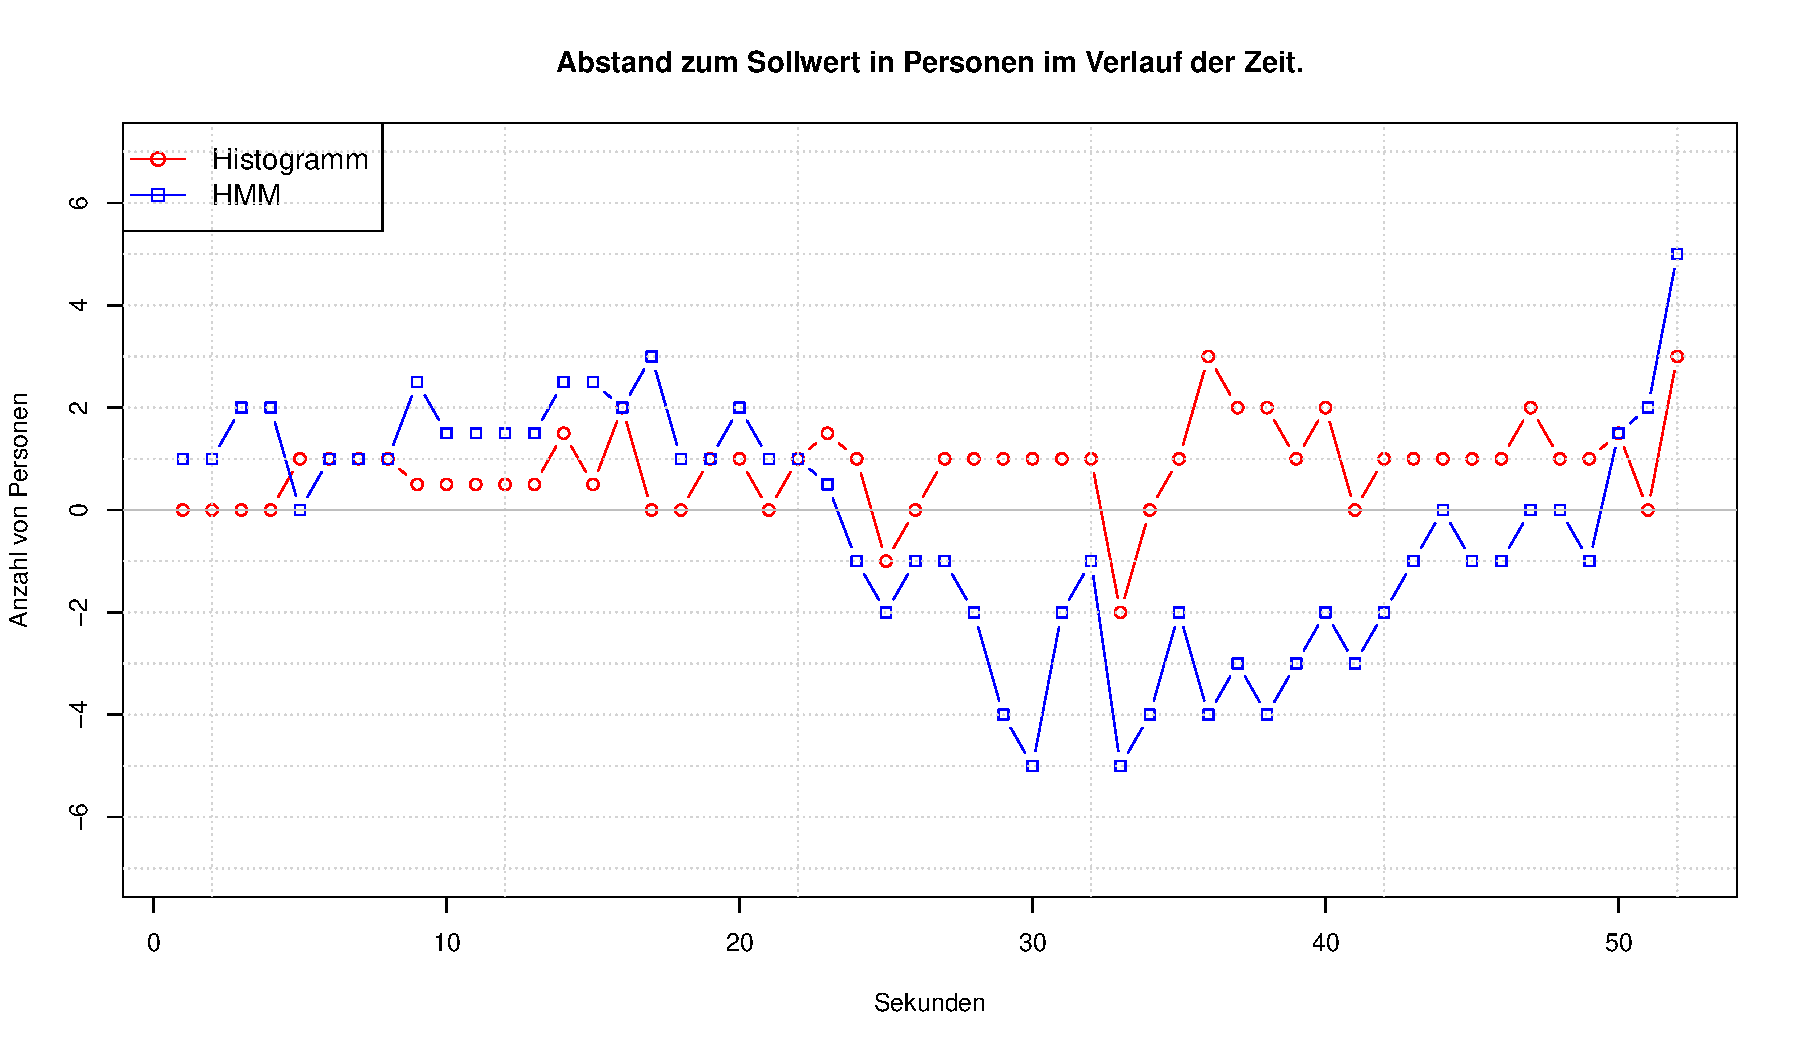
\includegraphics[width=1\textwidth]{bilder/innenhof_910-1000_histo_vs_hmm_prelearned.pdf}
\caption{Innenhof: Histogramm vs. trainiertes HMM}
	\label{fig:Innenhof}
\end{figure}

Abbildung \ref{fig:Innenhof} zeigt auf, dass der Histogramm-basierte Algorithmus für dieses Video durchgehend bessere Ergebnisse liefert, als der HMM-basierte Algorithmus. Der HMM-Algorithmus ist im Durchschnitt 1-2 Personen weiter vom realen Wert entfernt als sein Konkurrent. Im Besonderen gilt dies für den zweiten Teil des Videos.

\subsection{Vergleich mit Histogramm-basierter Implementierung: Tegel}
\label{sec:eval:tegel}

\begin{figure}
	\centering
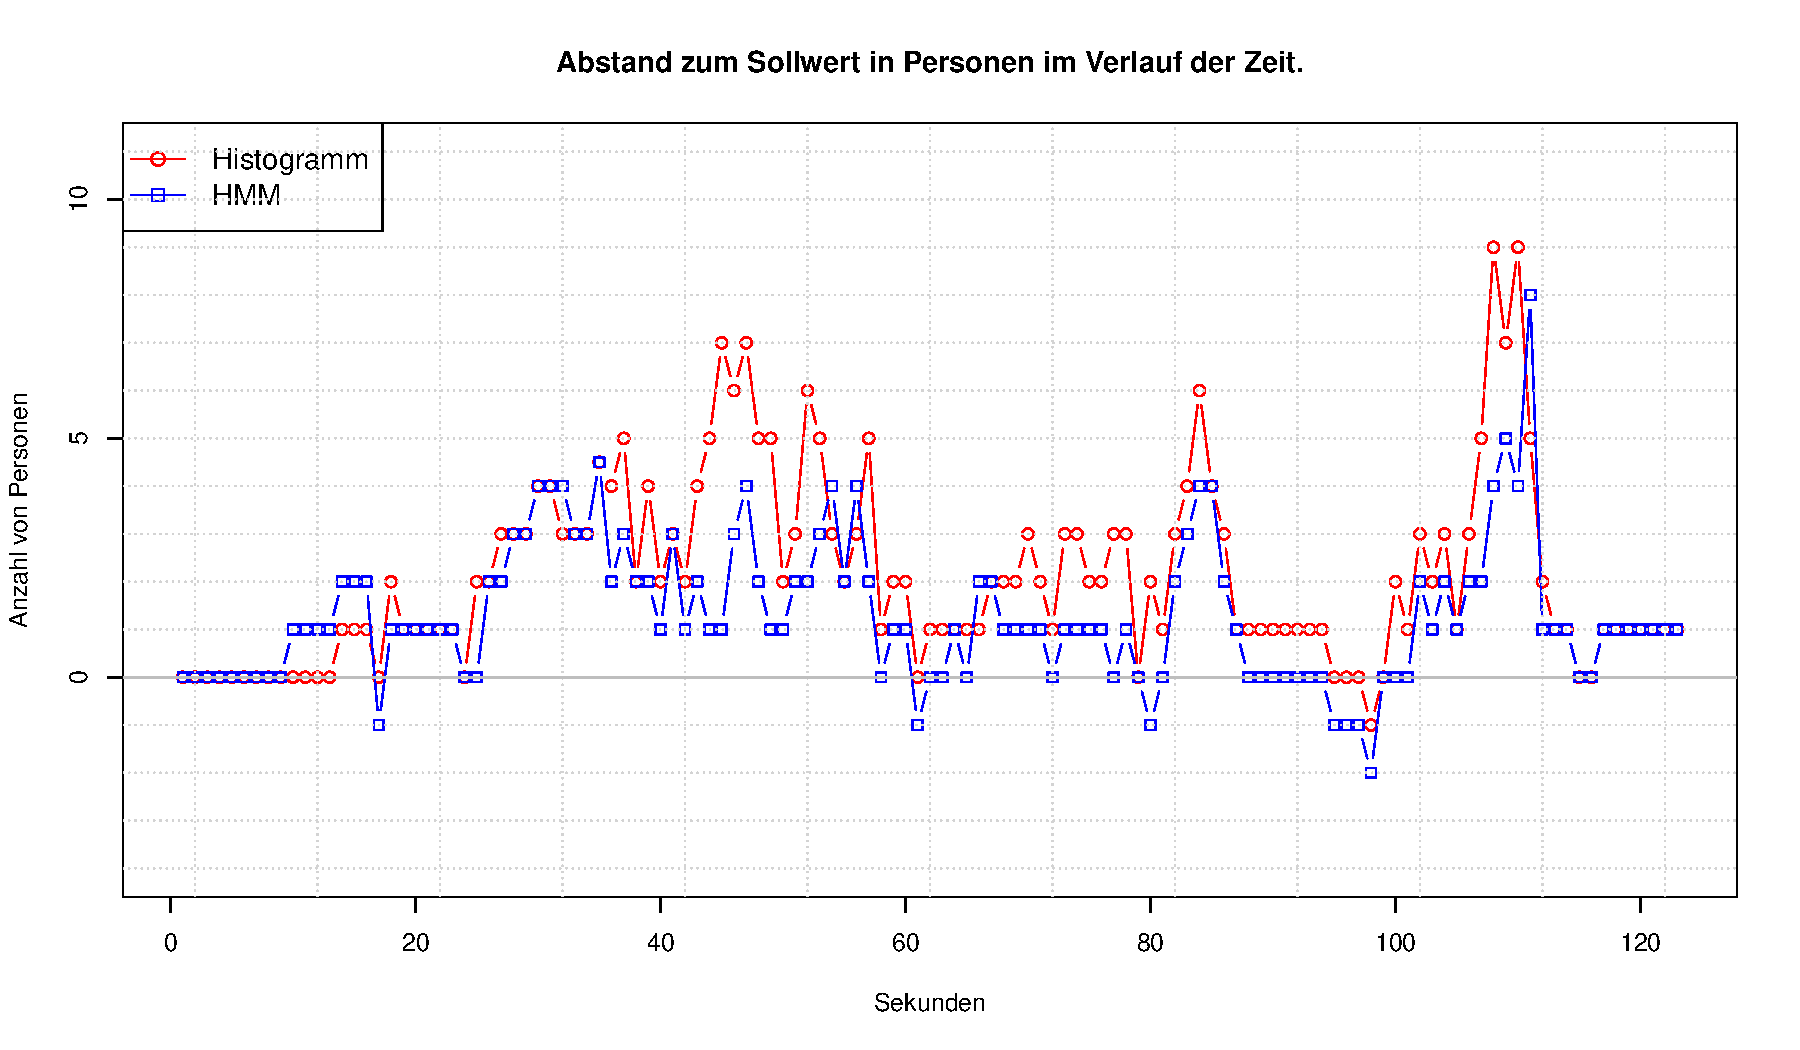
\includegraphics[width=1\textwidth]{bilder/tegel_7-55_histo_vs_prelearned_hmm.pdf}
	\caption{Tegel: Histogramm vs. trainiertes HMM}
	\label{fig:tegel}
\end{figure}

Wie man der Abbildung \ref{fig:tegel} entnehmen kann, sind die Ergebnisse beider Algorithmen vom Verlauf her sehr ähnlich, allerdings weist der HMM-basierte Algorithmus gegenüber dem Histogramm-basierten kleine Vorteile auf.
Zwischen 30 und 50 Sekunden hat er eine deutlich geringere Abweichung vom korrekten Wert. Dasselbe gilt für den Bereich zwischen ca. 65 und 80 Sekunden.\\

\subsection{Vergleich mit Histogramm-basierter Implementierung: Eingang}
\label{sec:eval_eingang}

\begin{figure}
	\centering
	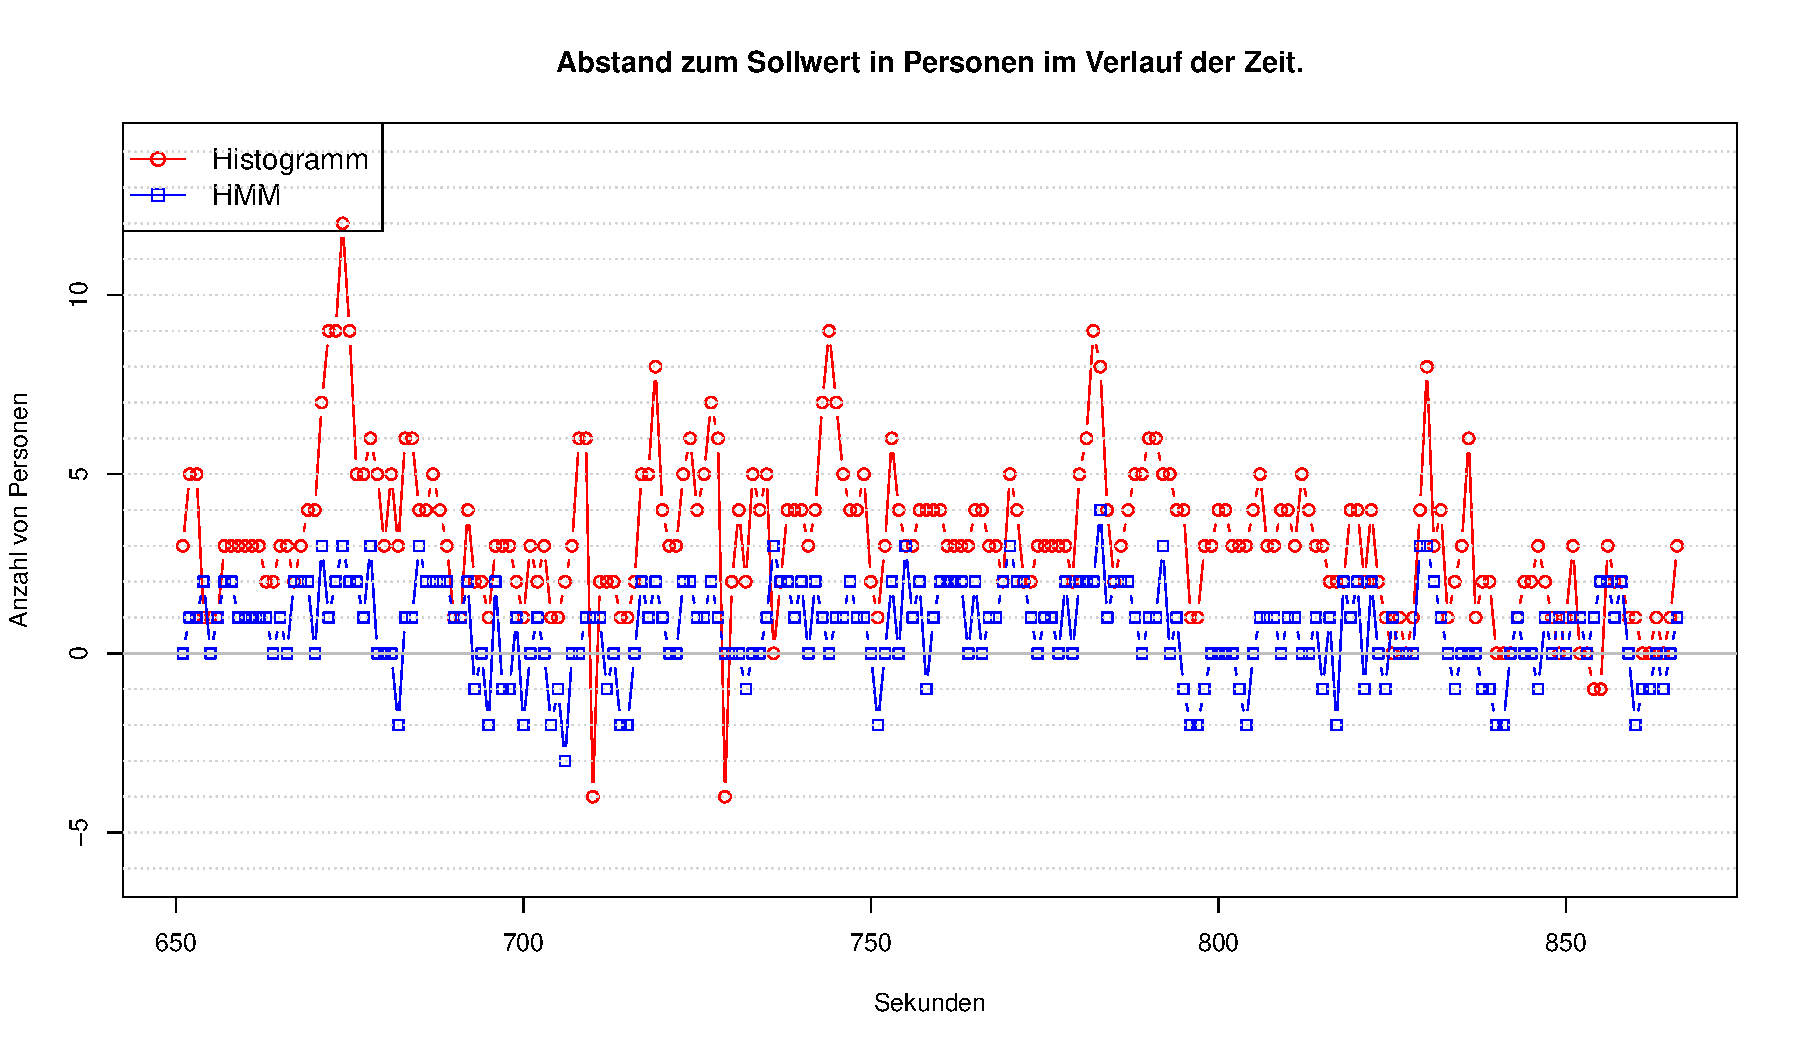
\includegraphics[width=1\textwidth {bilder/eingang2_histo_vs_hmm_prelearned.pdf}
	\caption{Eingang: Histogramm vs. trainiertes HMM (gesamt)}
	\label{fig:Eingang-gesamt}
\end{figure}

\begin{figure}
	\centering
	\includegraphics[width=1\textwidth]{bilder/safest_plot_histo_vs_prelearned_652-end.pdf}
	\caption{Eingang: Histogramm vs. trainiertes HMM, Ausschnitt Sekunde 651-Ende}
	\label{fig:Eingang-teil}
\end{figure}

In der Abbildung \ref{fig:Eingang-gesamt} erkennt man anhand der deutlich stärkeren Abweichung, dass beide Algorithmen Probleme mit der zuverlässigen Vordergrundextraktion haben.\\
Während in der ersten Hälfte des Videos der Histogramm-basierte Algorithmus noch Vorteile hat (relativ viele korrekte Anzeigen, der HMM-basierte Algorithmus erkennt meist eine Person zu viel), ist der HMM-basierte Algorithmus in der zweiten Hälfte des Videos (ab etwa Sekunde 450) deutlich besser. Wie der Grafik \ref{fig:Eingang-teil} zu entnehmen ist, existieren wesentlich weniger Ausreißer und das Ergebnis ist insgesamt auch viel dichter am korrekten Wert.\\

\subsection{Diskussion}
\label{sec:diskuss}
Aus den vorangehenden Grafiken kann man ablesen, dass beide Algorithmen grundsätzlich dazu geeignet sind, Vorder- von Hintergrund zu trennen. Sie besitzen jedoch Vor- und Nachteile in bestimmen Szenerien. Genau jene Unterschiede und Details müssen näher beschrieben und erklärt werden.

Wie aus Grafik \ref{fig:Eingang-gesamt} und \ref{fig:Eingang-teil} (Eingang) hervorgeht, besitzt der von uns entwickelte HMM-basierte Algorithmus besonders bei schwierigen, das heißt heterogenen, Hintergründen Vorteile bei der Erkennung. Trotz des hellen Hintergrunds, der viele Kanten und der häufigen Neukalibrierung der Kamera ist eine Erkennung mit kaum Ausreißern möglich. Dies liegt darin begründet, dass sich die Dynamik und die Veränderungen des Videobildes durch einen langen Lernprozess mitteln und des Weiteren Vordergrund nicht anhand von einfachen Grauwerten sondern anhand der komplexen (von uns eingeführten) Emissionen und den Übergängen zwischen ihnen erkannt wird.

Liegt jedoch ein homogener Hintergrund vor, so kann gesagt werden, dass beide Algorithmen gut funktionieren, jedoch ist in dieser Situation der Histogramm-basierte Algorithmus besser. Das liegt daran, dass der Hintergrund einen bestimmten Grauwert besitzt und auch Personen in ein ganz spezielles Intervall der Grauwerte fallen. Demnach arbeitet hier der Histogramm-basierte Algorithmus sehr effizient, unser Algorithmus unterliegt in dieser Domäne.

Den größten Vorteil hat der Histogramm-basierte Algorithmus bei der Performance: während dieser mit 22-25 fps eine flüssige Videodarstellung ermöglicht, lief der HMM-basierte Algorithmus nur mit ca. 10-12 fps. Hier wäre also noch Potential zur Verbesserung bei unserem Algorithmus.\\
Leider hat sich im Laufe des Projekts gezeigt, dass CvHMM sehr ineffizient auf einzelne Daten zugreift und die Ursache hierfür ist. Dies konnten wir mit Hilfe von Callgrind (Teil von Valgrind) nachweisen. Ein weiterer großer Nachteil von CvHMM ist, dass nur eine begrenzte Anzahl von Algorithmen Angeboten wird. Es fehlt der Forward-Algorithmus, den wir mit Hinblick auf die Performance dem ineffizienteren Viterbi-Algorithmus vorziehen würden. Auch haben die Veränderungen an der Netzwerktopologie keine Veränderungen am Resultat ergeben, was wir auf die Implementierung des Baum-Welch-Algorithmus in CvHMM zurückführen. Somit konnte nicht überprüft werden, ob die von uns verwendeten zwei Zustände optimal waren.

Zusätzlich sei angemerkt, dass außer im Falle der Grafik \ref{fig:Innenhof} (Innenhof) die Verläufe beider Graphen sehr ähnlich sind. Dies legt nahe, dass die vorliegenden Fehler eine gemeinsame Ursache besitzen. Diese Ursache konnte von uns teilweise lokalisiert werden: das Clustering, welches markierten Vordergrund in die Anzahl von Personen übersetzt, ist oft zu großzügig. Wir konnten beobachten, dass bei den Tegel- und Eingang-Videos einzelne Personen in zwei oder mehr Cluster (Personen) geteilt werden.

Unseren Ergebnissen nach bewerten wir unser Algorithmus als einen allgemein einsatzfähigen Algorithmus, der in allen Szenerien gut genug ist (ein \glqq allrounder \grqq{}) der gegenüber dem spezialisierten Histogramm-basierten Ansatz in manchen Szenerien besser, in manchen schlechter abschneidet, aber stets gut genug ist.
\section{Fazit und Ausblick}
\label{chap:fazit}

% ausblick
Wir sehen unsere Ziele der Anforderungsanalyse aus Kapitel \ref{sec:anforderungsanalyse} als erfüllt. Die in dem Abschnitt \ref{sec:diskuss} angesprochenen Nachteile können sehr wahrscheinlich überwunden werden, wobei die Verwendung einer besseren Bibliothek für HMMs die erste wichtige Anpassung sein sollte. Ein möglicher Kandidat für eine bessere HMM-Bibliothek wäre dabei HMMlib\cite{hmmlib}, welches deutlich auf Performance hin optimiert wurde und des Weiteren den Forward-Algorithmus anbietet. Je nach eingesetzter Hardware kann auch Threading verwendet werden, um durch eine Einteilung des Bildframes in Bereiche und nichtsequentielle Berechnung die Abarbeitung zu beschleunigen. Zudem sollten algorithmische Anpassungen und theoretische Untersuchungen überprüfen, wie groß der Einfluss einer anderen HMM-Topologie wäre.


%Fazit
Wir werten das Ergebnis unseres Projekts als Erfolg. Wir haben nachgewiesen, dass es möglich ist, einen auf HMM-basierenden Algorithmus zur Trennung von Vorder- und Hintergrund zu verwenden und haben mit diesen ähnlich gute Ergebnisse erzielt, wie mit den bereits implementierten Algorithmen. Bei heterogenen Hintergründen besitzt unser Konzept klare Vorteile gegenüber den Histogramm-basierten Algorithmus. Zusammenfassend erscheint der Einsatz eines HMM-basierten Vordergrundextraktors als sinnvoll.

%  [habe ich zunächst ausgelassen, da ghosting imho problem von zu hochfrequenten lernens war, nicht von zu kurzen videos]

% Interessant wäre zudem, ob es möglich ist, eine sinnvolle online-Lernfähigkeit zu integrieren, wenn die verwendeten Videosequenzen lang genug sind (was im Falle von realen Überwachungskameras ja kein Problem darstellen würde).
%Allerdings haben wir nur \glqq Offline-Learning\grqq{} genutzt, da die uns zur Verfügung gestellten Sequenzen für \glqq Online-Learning\grqq{} zu kurz waren. Wenn wir versucht haben, online zu lernen, führte dies immer zu schlechteren Ergebnissen aufgrund von Geisterbildern.\\

%[ausgleassen da dperciated und die die super starke hardware erstmal egal ist...]

 %oder vielleicht sogar die, wie wir später herausgefunden haben, in OpenCV enthaltenen HMM-Funktionen, die allerdings innerhalb des OpenCV-Projekts nicht weiterentwickelt werden und derzeit des Status “deprecated” haben. %Gerade HMMlib ist sehr viel mehr auf Performance optimiert, setzt dafür aber auch stärkere Hardware vorraus (SSE3). 



\nocite{lamarre2002tracking}

\newpage

\printbibliography

\end{document}
